\documentclass[12pt,letter]{article}
\usepackage{mathptmx} % added for time new roman font
\usepackage[left=1in,right=1in,top=1in,bottom=1in]{geometry}
\usepackage[latin1]{inputenc}
\usepackage{amsmath}

% defines all example enviorment
\usepackage[framemethod=tikz]{mdframed} % added for the box around examples
\newtheorem{ex}{Example}
\numberwithin{ex}{section} % allows for the use of example numbers that lign up with the section numbers
\newenvironment{example}{\begin{mdframed}[middlelinewidth=0.5mm]\begin{ex}\normalfont}{\end{ex}\end{mdframed}}

% defines all review enviorment
\usepackage[framemethod=tikz]{mdframed} % added for the box around examples
\newtheorem{re}{Review}
\numberwithin{re}{section} % allows for the use of example numbers that lign up with the section numbers
\newenvironment{review}{\begin{mdframed}[middlelinewidth=2mm,roundcorner=20pt]\begin{re}\normalfont}{\end{re}\end{mdframed}}

% defines the quotation enviorment 
\usepackage{xcolor}
\newcommand{\quotebox}[2]{\begin{center}\fcolorbox{white}{blue!15!gray!15}{\begin{minipage}{0.9\linewidth}\vspace{10pt}\center\begin{minipage}{0.8\linewidth}{\space\Huge``}{#1}{\Huge''}{\break\null\hfill} {\small #2}  \end{minipage}\medbreak\end{minipage}}\end{center}}

% defines the definition enviorment 
\newcommand{\definitionbox}[2]{\begin{center}\fcolorbox{white}{blue!15!gray!15}{\begin{minipage}{0.9\linewidth}\vspace{10pt}\center\begin{minipage}{0.8\linewidth} {{\textbf{Definition} - }{#1}: {#2}}\end{minipage}\medbreak\end{minipage}}\end{center}}

\usepackage{amsfonts}
\usepackage{amssymb}
\usepackage{graphicx}
\usepackage{float}
\usepackage{booktabs}
%\usepackage{parskip} % remove all the paragraph indents

\usepackage{setspace}
%\usepackage[colorlinks=true]{hyperref}
\usepackage{textcomp} 
\usepackage{multicol} 


%%%%%%%		define the symbols for positive directions		%%%%%%
\makeatletter													%%	
																%%					
\newcommand*\curveplus{% positive counterclockwise				%%
  \mathbin{\rotatebox[origin=c]{90}{$\m@th\curvearrowleft$}+}}	%%
																%%
\newcommand*\rightplus{% positive right							%%
  \mathpalette\@rightplus\relax}								%%
\newcommand*\@rightplus[1]{%									%%
  \mathbin{\vcenter{\hbox{$\m@th\overset{#1+}{\to}$}}}}			%%
																%%	
\newcommand*\upplus{% positive up								%%
  \mathbin{+\mathord\uparrow}}									%%
																%%			
\newcommand*\downplus{% positive down							%%		
  \mathbin{+\mathord\downarrow}}								%%
  																%%		
\newcommand*\downrightplus{% positive down and right			%%	
  \mathbin{+ \rotatebox[origin=c]{-30}{$\m@th\rightarrow$}}}	%%
\makeatother 													%%	
%%%%%%%%%%%%%%%%%%%%%%%%%%%%%%%%%%%%%%%%%%%%%%%%%%%%%%%%%%%%%%%%%%


\usepackage{mathtools}          %loads amsmath as well added for the piece wise function
\DeclarePairedDelimiter\Floor\lfloor\rfloor
\DeclarePairedDelimiter\Ceil\lceil\rceil

 
\newcounter{NumberInTable}
\newcommand{\LTNUM}{\stepcounter{NumberInTable}{(\theNumberInTable)}}

\newcommand{\Laplace}[1]{\ensuremath{\mathcal{L}{\left[#1\right]}}}
\newcommand{\InvLap}[1]{\ensuremath{\mathcal{L}^{-1}{\left[#1\right]}}}
\renewcommand{\textuparrow}{$\uparrow$}


\begin{document}



\setcounter{section}{5}	
\section{Vibration Control}

Throughout this text, we have studied various aspects related to analyzing and modeling vibrating systems. Therefore, it becomes prudent to look at methods for reducing or eliminating unwanted vibrations. However, before vibrations in a system can be effectively reduced they must be better understood in terms of their effects on the system under study. For this reason, this chapter first introduces the vibration Nomograph, this is then followed by vibration isolation, absorption, and active suppression.  

\subsection{Vibration Nomograph}

There exist various methods and standards for measuring and describing acceptable levels of vibrations in systems, these include ISO/AWI 2631 for the evaluation of human exposure to whole-body vibrations and ISO 4866 for the measurement and effects of vibrations on structures. A common way to present the acceptable limit of vibration is in a vibration nomograph.  A vibration nomograph is a simplified way to express the acceptable limits on a system while considering the displacement, velocity, acceleration, and frequency of a system. A typical nomograph with various limits is presented in figure \ref{fig:Vibration_nomograph}. 

A vibration nomograph is a logarithmic plot that allows us to easily express the relationships between displacement, velocity, acceleration, and frequency of a system. The vibration nomograph presented in figure \ref{fig:Vibration_nomograph} considers an undamped 1-DOF system with constant amplitude ($A$) experiencing harmonic motion that can be modeled as:
\begin{equation}
    x(t) = A \sin(\omega t)
    \label{eq:displacement}
\end{equation}
Therefore, the velocity and acceleration terms can be found by taking the derivatives of the displacement expression to yield:
\begin{equation}
    \dot{x}(t) = A \omega \cos(\omega t)
\end{equation}
and:
\begin{equation}
    \ddot{x}(t) = -A\omega^2 \sin(\omega t)
    \label{eq:acceleration}
\end{equation}
These equations are converted from a circular frequency in rad/sec to a linear frequency ($f$) in Hz, such that $\omega = 2\pi f$. Therefore, equations \ref{eq:displacement}-\ref{eq:acceleration} become:
\begin{equation}
    x(t) = A \sin(\omega t)
\end{equation}
\begin{equation}
    v(t) =  \dot{x}(t) = 2\pi f A \cos(\omega t)
\end{equation}
\begin{equation}
    a(t) =  \ddot{x}(t) = -4\pi^2 f^2 A \sin(\omega t)
\end{equation}
Thereafter, the maximum values for velocity $v_\text{max}$ and acceleration $a_\text{max}$ are related to amplitude through:
\begin{equation}
    v_\text{max} = 2\pi f A 
    \label{eq:v_max}
\end{equation}
\begin{equation}
    a_\text{max} = -4\pi^2 f^2 A = -2 \pi f v_\text{max}
    \label{eq:a_max}
\end{equation}
by taking the natural log of both side of equation \ref{eq:v_max} we obtain: 
\begin{equation}
    \ln v_\text{max} = \ln 2 \pi f + \ln A
    \label{eq:ln_v_max} 
\end{equation}
doing the same for equation \ref{eq:a_max} and rearranging in terms of $v_\text{max}$ leads to:
\begin{equation}
    \ln v_\text{max} = - \ln a_\text{max} - \ln 2\pi f  
    \label{eq:ln_v_max_2} 
\end{equation}
It can be seen that both of these expressions are linear. Moreover, for a constant amplitude of displacement, $A$, equation \ref{eq:ln_v_max} tells us that $\ln v_\text{max}$ varies with $\ln (2 \pi f)$. As the $x-$axis in a nomograph is frequency, measured in Hz, $\ln (2 \pi f)$ is a straight line with a positive slope of 1. Therefore, a line on the nomograph that represents a constant displacement is at a 45$^\circ$ angle from the $x$-axis. Similarly, equation \ref{eq:ln_v_max_2} shows that for a constant value of acceleration ($a_\text{max}$) the $\ln v_\text{max}$ is represented by a straight line that varies with $- \ln(2\pi f)$, therefore,  $\ln v_\text{max}$ is a straight line with the slope of -1. This is also represented by a line of constant acceleration set at a -45$^\circ$ angle from the $x$-axis. These equations are expressed in the vibration nomograph plot of figure \ref{fig:Vibration_nomograph} where each point on the plot represents a specific sinusoidal (harmonic) vibration for a 1-DOF system.  

\begin{figure}[H]
    \centering
    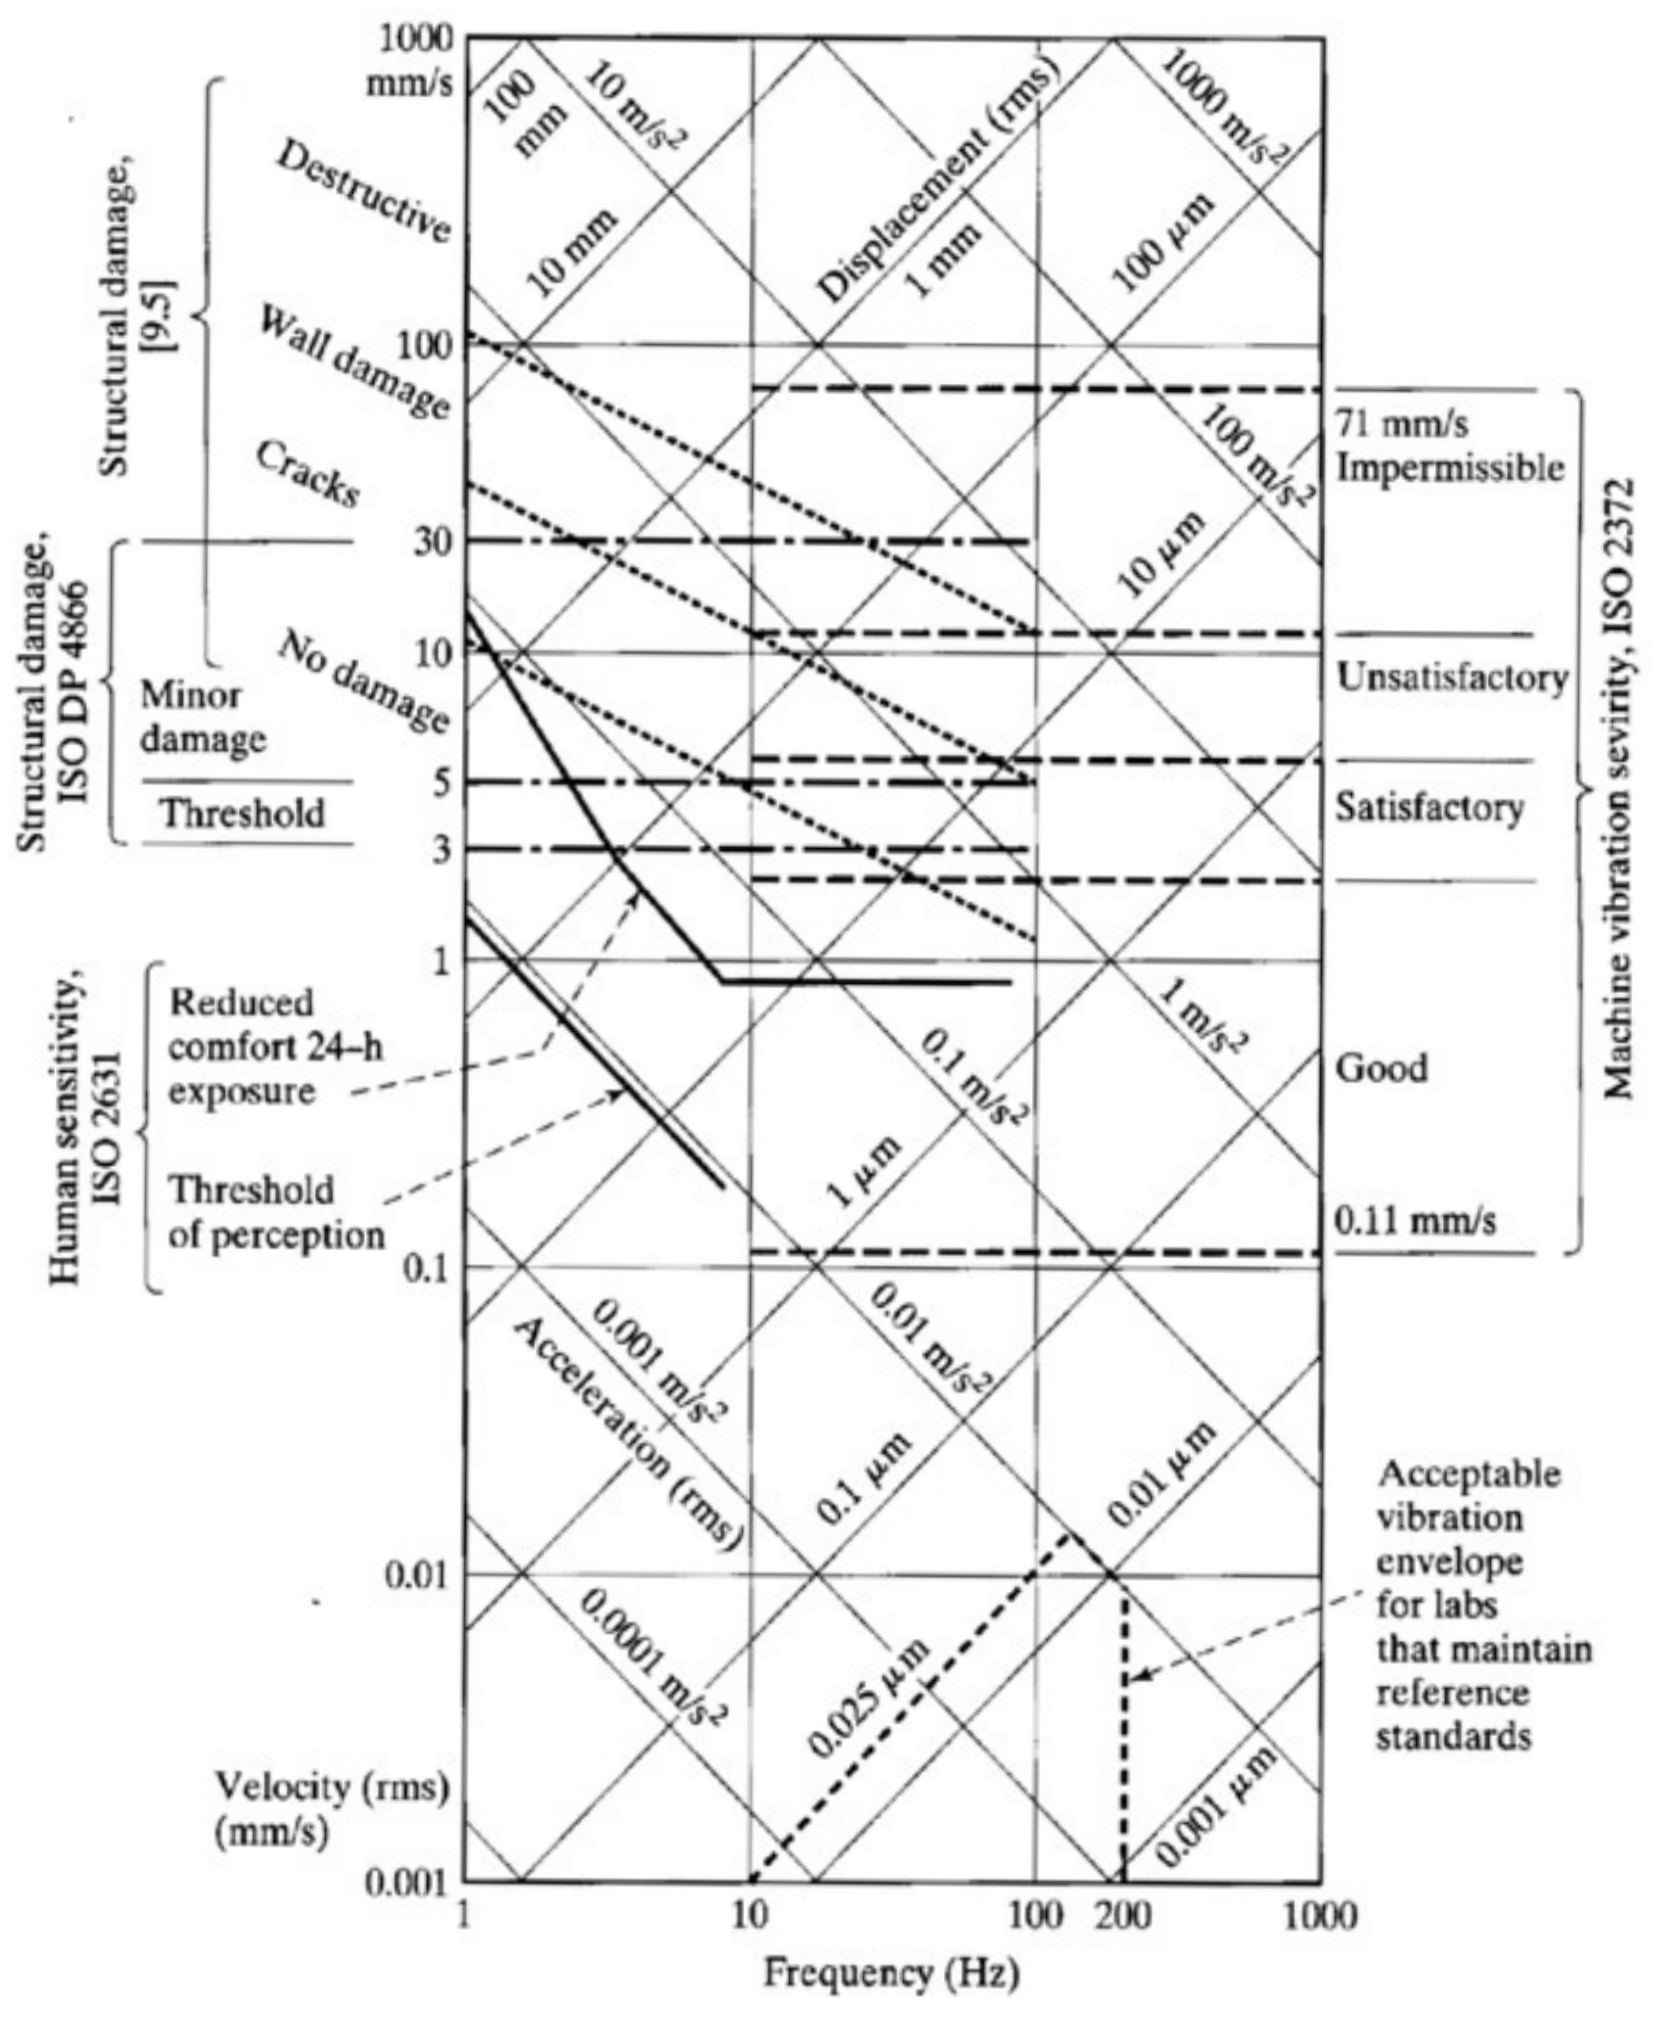
\includegraphics[width=5in]{../Figures/Vibration_nomograph.png}
    \caption{Vibration nomograph showing the acceptable limits of vibration for various applications. Adopted from \cite{Rao2017Mechanicalvibrations} and \cite{Macinante1984Seismicmountingsvibration}.}
    \label{fig:Vibration_nomograph}
\end{figure}


\subsection{Vibration Isolation}



\subsection{Vibration Absorption}



\subsection{Active Vibration Suppression}

Active vibration control add energy to the system in order to mitigate the vibrations in the system. As depicted in figure \ref{fig:active_vibration_control_FBD}(a), an active vibration control system requires a sensor to acquire data from the system, control hardware and algorithms to processes this data, and an actuator to exert a physical control on the system. These system together are called a feedback loop, as a movement in the mass results in a control force $(f_u)$ being exerted on the system. This control force is diagrammed in figure \ref{fig:active_vibration_control_FBD}(b). 

\begin{figure}[H]
    \centering
    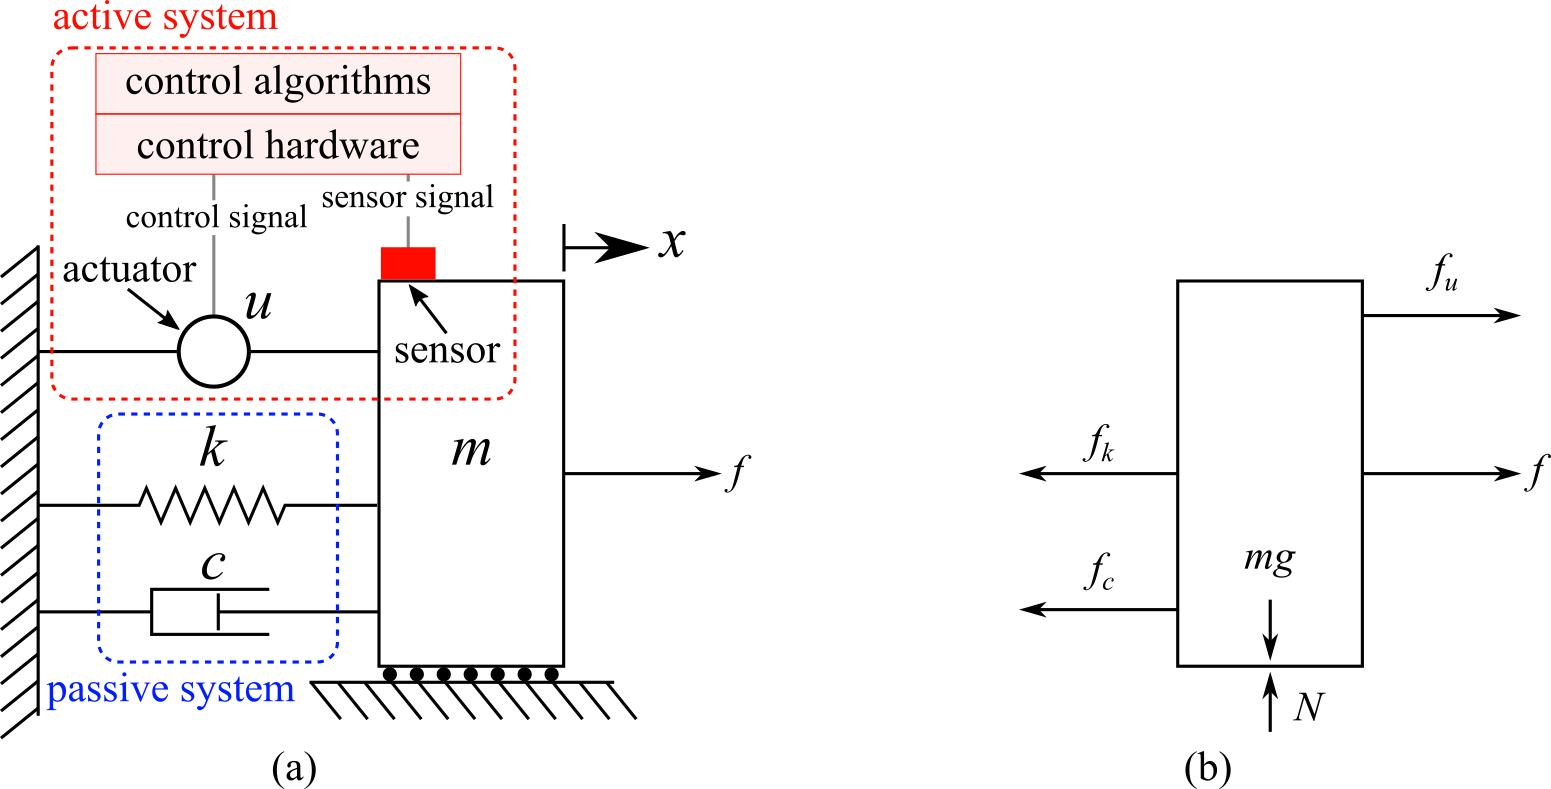
\includegraphics[width=5in]{../Figures/active_vibration_control_FBD.png}
    \caption{Active vibration control system showing: (a) the system with a feed-back loop that takes a signal from the sensor, converts it to a control signal, and drives the actuator; and (b) the free body diagram.}
    \label{fig:active_vibration_control_FBD}
\end{figure}

Adding the control force to the EOM for the 1-DOF system presented in figure \ref{fig:active_vibration_control_FBD} results in:
\begin{equation}
m \ddot{x} + c \dot{x} + kx = F(t) = f + f_u
\end{equation}
A common method for providing control for vibration suppression is called position derivative control or PD-control. PD-control measures the position and velocity of the mass and uses these to compute the control force needed to mitigate the vibration to an acceptable level. A simple way to code a PD-controller is to provide a control force proportional to the displacement velocity (derivative of displacement) of the mass such that:
\begin{equation}
f_u = -g_1x - g_2 \ddot{x}
\end{equation}
where $g_1$ and $g_2$ are the proportional gains of the systems. The control gains can be constants determined by the designer or variables updated through time by an algorithm. Here we will consider the gains to be constant, therefore, the EOM for the closed-loop system in figure \ref{fig:active_vibration_control_FBD} becomes:
\begin{equation}
m \ddot{x} + (c + g_2) \dot{x} + (k + g_1)x = F(t) = f 
\end{equation}
This formulation lets $g_1$ act as additional damping while $g_2$ acts as additional damping. This closed-loop EOM can be used to solve for the effective natural frequency of the system, given by:
\begin{equation}
\omega_n = \sqrt{\frac{k+g_p}{m}}
\end{equation}
and the effective damping ratio of the system
\begin{equation}
\zeta = \frac{c+g_2}{2\sqrt{m(k+g_1)}}
\end{equation}



























			\noindent
			

	\pagebreak
	\renewcommand{\thepage}{}
	\renewcommand\refname{References Cited}
	\pagestyle{plain}
	\bibliographystyle{unsrtDOI}
	\bibliography{Chapter_6_vibration_control}
	
\end{document}














